\documentclass[12pt,article]{article}
\usepackage{fullpage}
\usepackage[top=2cm, bottom=4.5cm, left=2cm, right=2cm]{geometry}
\usepackage{amsmath,amsthm,amsfonts,amssymb,amscd}
\usepackage{lastpage}
\usepackage{enumerate}
\usepackage{fancyhdr}
\usepackage{mathrsfs}
\usepackage{xcolor}
\usepackage{graphicx}
\usepackage{wrapfig}
\usepackage[font=scriptsize]{caption}
\usepackage{listings}
\usepackage{hyperref}
\usepackage{mdframed}
\usepackage{changepage}   % for the adjust width environment
\usepackage{forest} 
\usepackage{tikz}   % For graph
\usepackage{float}  % To in force inserting images at the right place
\usepackage{geometry}
\usepackage{array}
\usepackage{icomma}
\newcolumntype{C}[1]{p{#1}}

\graphicspath{ {./images/} }

\newcommand{\Tau}{\mathrm{T}}



% For matrix
\def\horzbar{\text{magic}}

\hypersetup{%
  colorlinks=true,
  linkcolor=blue,
  linkbordercolor={0 0 1}
}

\setlength{\parindent}{0.0in}
\setlength{\parskip}{0.05in}
%\addtolength{\tabcolsep}{-2pt}

\newcommand\projnumber{4}
\newcommand\course{CS534}
\newcommand\OSUID{934370552}
\newcommand\Email{buivy@oregonstate.edu}
\newcommand\Name{Vy Bui}
\newcommand\tab[1][1cm]{\hspace*{#1}}

\pagestyle{fancyplain}
\headheight 35pt
\lhead{Implementation Assignment \projnumber}
%\rhead{Oct. 20, 2022}
\rhead{\small\thepage}
\lfoot{}
\cfoot{}
\headsep 1.5em

\newenvironment{problem}[2][Problem]
    { \begin{mdframed}[backgroundcolor=gray!20] \textbf{#1 #2} \\}
    {  \end{mdframed}}
   
% Make Right arrow with superscript
\makeatletter
\newcommand{\xRightarrow}[2][]{\ext@arrow 0359\Rightarrowfill@{#1}{#2}}
\makeatother

\begin{document}

\begin{titlepage}
    \begin{center}
        \vspace*{4cm}

        \textbf{\Large CS534 - Machine Learning}

        \vspace{0.5cm}
 
        \textbf{\Large Implementation Assignment \projnumber{}}
 
        \vspace{1cm}

        \textbf{Group 50}

        Sebastian Mueller - 933962290

        Derek Helms - 934451909

        Vy Bui - 934370552
        
        

        \vspace{2cm}

        \textbf{Instructor: Dr. Xiaoli Fern}
        \vfill
             
        \vspace{0.8cm}
      
             
        The School of Electrical Engineering and Computer Science\\
        Oregon State University\\
        \vspace{3pt}
        Nov 22, 2022     
    \end{center}
\end{titlepage}

\newpage

\begin{center} \Large{\textbf{Word Embedding Exploration }} \end{center}
\textbf{Question 1:}\newline
list the 29 most similar words
for each seed word.\newline

\textbf{Response:}\newline

    \begin{minipage}[c]{0.25\linewidth}%
        \scalebox{0.9}{
        \begin{tabular}{|c|c|}
           \hline
           \textbf{rank} & \textbf{word} \\
           \hline
            1 &  plane \\
            \hline
            2 &  flights \\
            \hline
            3 & boarding  \\
            \hline
            4 &  airline \\
            \hline
            5 &  jet \\
            \hline
            6 &  flying\\
            \hline
            7 &  heading\\
            \hline
            8 &  arrival \\
            \hline
            9 &  airlines \\
            \hline
            10 &  travel \\
            \hline
            11 &  shuttle\\
            \hline
            12 &  delayed \\
            \hline
            13 &  landing \\
            \hline
            14 &  route \\
            \hline
            15 &  airplane\\
            \hline
            16 &  safe \\
            \hline
            17 &  booking \\
            \hline
            18 &  fly \\
            \hline
            19 &  departure\\
            \hline
            20 &  waiting\\
            \hline
            21 &  landed\\
            \hline
            22 &  journey\\
            \hline
            23 &  passengers\\
            \hline
            24 &  transit\\
            \hline
            25 &  delay\\
            \hline
            26 &  crew\\
            \hline
            27 &  pilot\\
            \hline
            28 &  trip\\
            \hline
            29 &  taxi\\
            \hline
    \end{tabular}}
    %\captionof{figure}{29 most similar \newline words to "flight"}
    \end{minipage}
    \hspace{-28pt}%
    \begin{minipage}[c]{0.25\linewidth}%
        \scalebox{0.9}{
        \begin{tabular}{|c|c|}
           \hline
           \textbf{rank} & \textbf{word}  \\
           \hline
            1 &  great \\
            \hline
            2 &  well \\
            \hline
            3 & nice  \\
            \hline
            4 &  better \\
            \hline
            5 &  night \\
            \hline
            6 &  bad\\
            \hline
            7 &  morning\\
            \hline
            8 &  way \\
            \hline
            9 &  hope \\
            \hline
            10 &  but \\
            \hline
            11 &  too\\
            \hline
            12 &  really \\
            \hline
            13 &  right \\
            \hline
            14 &  through \\
            \hline
            15 &  there\\
            \hline
            16 &  day \\
            \hline
            17 &  luck \\
            \hline
            18 &  sure \\
            \hline
            19 &  it \\
            \hline
            20 &  thing \\
            \hline
            21 &  pretty \\
            \hline
            22 &  think \\
            \hline
            23 &  have \\
            \hline
            24 &  all \\
            \hline
            25 &  yes \\
            \hline
            26 &  very \\
            \hline
            27 &  again\\
            \hline
            28 &  work\\
            \hline
            29 &  yeah\\
            \hline
    \end{tabular}}
     %\captionof{figure}{29 most similar\newline words to "good"}
    \end{minipage}
    \hspace{-37pt}%
    \begin{minipage}[c]{0.25\linewidth}%
        \scalebox{0.9}{
        \begin{tabular}{|c|c|}
           \hline
           \textbf{rank} & \textbf{word}  \\
           \hline
            1 &  horrible  \\
            \hline
            2 &  awful \\
            \hline
            3 & bad  \\
            \hline
            4 &  brutal \\
            \hline
            5 &  idea \\
            \hline
            6 &  horrendous \\
            \hline
            7 &  horrid \\
            \hline
            8 &  shitty \\
            \hline
            9 &  quite \\
            \hline
            10 &  worst \\
            \hline
            11 &  similar \\
            \hline
            12 &  shame \\
            \hline
            13 &  worse \\
            \hline
            14 &  crap \\
            \hline
            15 &  actual \\
            \hline
            16 &  horrific \\
            \hline
            17 &  bloody \\
            \hline
            18 &  ridiculous \\
            \hline
            19 &  such \\
            \hline
            20 &  atrocious \\
            \hline
            21 &  dreadful \\
            \hline
            22 &  sick \\
            \hline
            23 &  wtf \\
            \hline
            24 &  fucking \\
            \hline
            25 &  cruel \\
            \hline
            26 &  seriously \\
            \hline
            27 &  unreal \\
            \hline
            28 &  mess \\
            \hline
            29 &  however \\
            \hline
    \end{tabular}}
    %\captionof{figure}{29 most similar \newline words to "terrible"}
    \end{minipage}
    \hspace{-22pt}%
    \begin{minipage}[c]{0.25\linewidth}%
        \scalebox{0.9}{
        \begin{tabular}{|c|c|}
           \hline
           \textbf{rank} & \textbf{word}  \\
           \hline
            1 &  need \\
            \hline
            2 &  helping \\
            \hline
            3 & please  \\
            \hline
            4 &  pls \\
            \hline
            5 &  let \\
            \hline
            6 &  us \\
            \hline
            7 &  give \\
            \hline
            8 &  trying \\
            \hline
            9 &  can \\
            \hline
            10 &  helps \\
            \hline
            11 &  must \\
            \hline
            12 &  tell \\
            \hline
            13 &  find \\
            \hline
            14 &  could \\
            \hline
            15 &  plz \\
            \hline
            16 &  helped \\
            \hline
            17 &  support \\
            \hline
            18 &  anyone \\
            \hline
            19 &  should \\
            \hline
            20 &  save \\
            \hline
            21 &  take \\
            \hline
            22 &  want \\
            \hline
            23 &  bring \\
            \hline
            24 &  maybe \\
            \hline
            25 &  lets \\
            \hline
            26 &  seriously \\
            \hline
            27 &  able \\
            \hline
            28 &  here \\
            \hline
            29 &  needs \\
            \hline
    \end{tabular}}
    %\captionof{figure}{29 most similar \newline words to "help"}
\end{minipage}
\hspace{-35pt}%
    \begin{minipage}[c]{0.25\linewidth}%
        \scalebox{0.9}{
        \begin{tabular}{|c|c|}
           \hline
           \textbf{rank} & \textbf{word}  \\
           \hline
            1 &  early \\
            \hline
            2 &  earlier \\
            \hline
            3 & usual  \\
            \hline
            4 &  after \\
            \hline
            5 &  again \\
            \hline
            6 &  saturday \\
            \hline
            7 &  afternoon \\
            \hline
            8 &  hour \\
            \hline
            9 &  guess \\
            \hline
            10 &  missed \\
            \hline
            11 &  work \\
            \hline
            12 &  hours \\
            \hline
            13 &  sunday \\
            \hline
            14 &  since \\
            \hline
            15 &  night \\
            \hline
            16 &  away \\
            \hline
            17 &  yesterday \\
            \hline
            18 &  last \\
            \hline
            19 &  maybe \\
            \hline
            20 &  yet \\
            \hline
            21 &  monday \\
            \hline
            22 &  wait \\
            \hline
            23 &  either \\
            \hline
            24 &  mins \\
            \hline
            25 &  wake\\
            \hline
            26 &  before\\
            \hline
            27 &  thursday\\
            \hline
            28 &  hopefully\\
            \hline
            29 &  friday\\
            \hline
    \end{tabular}}
    %\captionof{figure}{29 most similar \newline words to "late"}
\end{minipage}% 
\newline

\protect{\scriptsize{Table 1: Tables from left to right display 29 most similar words to words "flight", "good", "terrible", "help", and "late" respectively.}}
\newline

\textbf{Question 2:}\newline
Do you observe five distinct clusters in your visualization?\newline
\newpage
\textbf{Response:}

\begin{figure}[H]
\centering
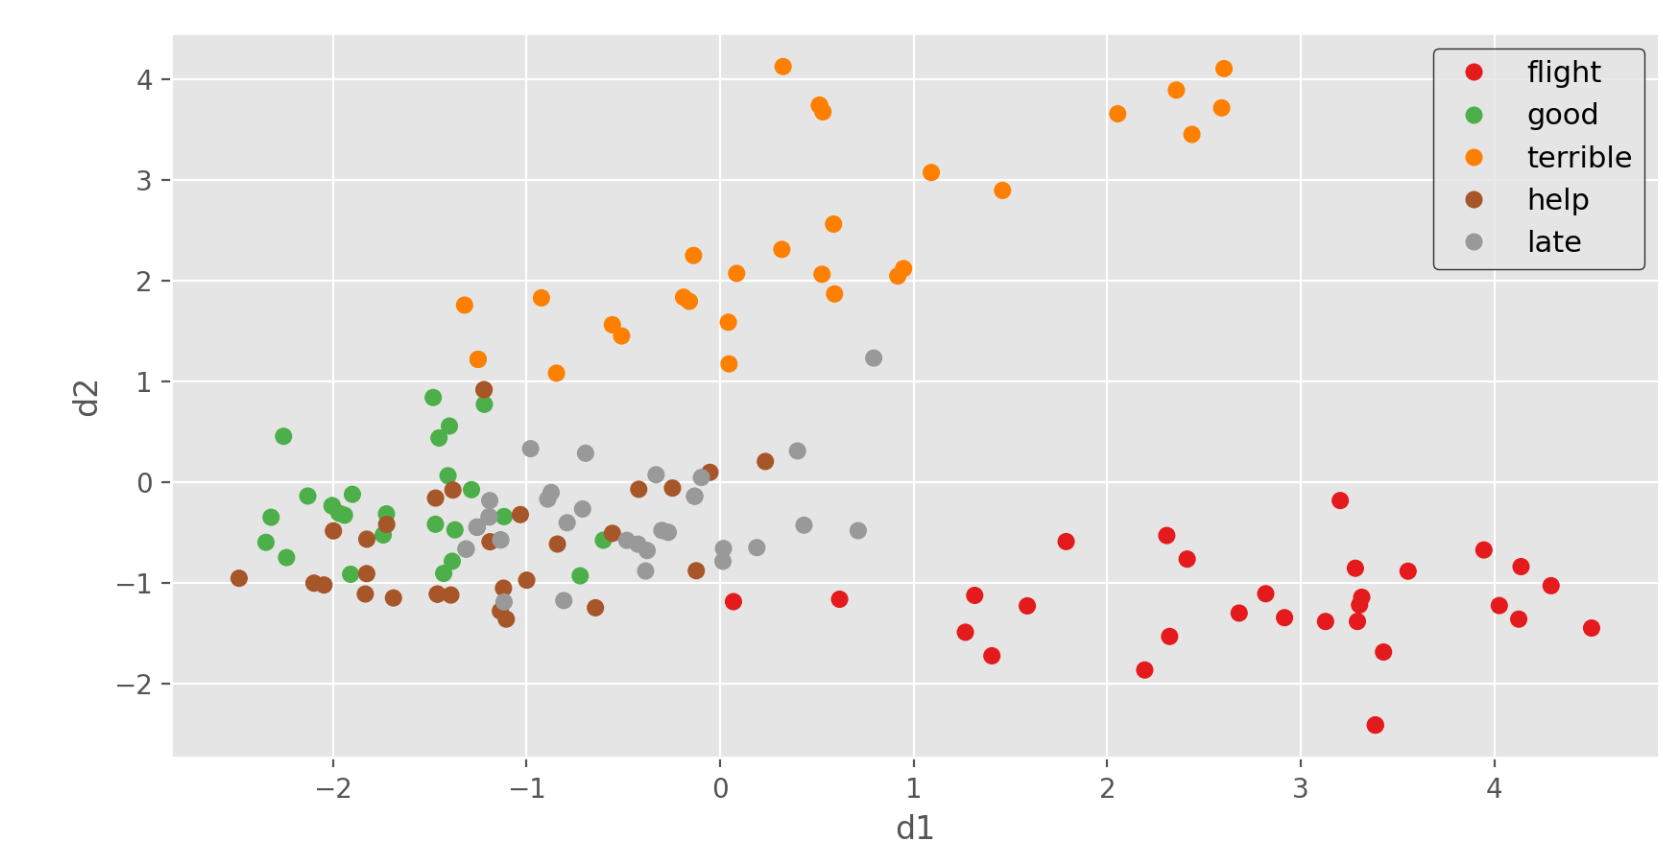
\includegraphics[scale = 0.35]{images/PCA_clusters.png}    
\captionsetup{labelformat=empty}
\vspace{-5pt}
\caption{\scriptsize{\;\;\;\;\;\;\;\;\;\;\;\;\;Figure 1: PCA on 150 Clustered Words}}
\end{figure}

We did not get five distinct clusters (Figure 1). There is an overlap between the words closest to "good", "help", "late". The words closest to "flight" and "terrible" have a clearer separation in the clusters.\newline

\textbf{Question 3:}\newline
Provide substantially different visualization results by using different perplexity parameter for t-SNE .\newline

\textbf{Response:}\newline
Figures 2 \& 3 showcase our exploration of different perplexity values. You can dramatic shifts in clustering tightness and location, even between successive increments sometimes. Such as in perplexity = 41 and perplexity = 43 in Figure 3. These changes could be caused by different initialization since t-SNE has non convex cost functions, which means it can get stuck in different local minimum. \newline
\newpage
\begin{figure}[H]
\centering
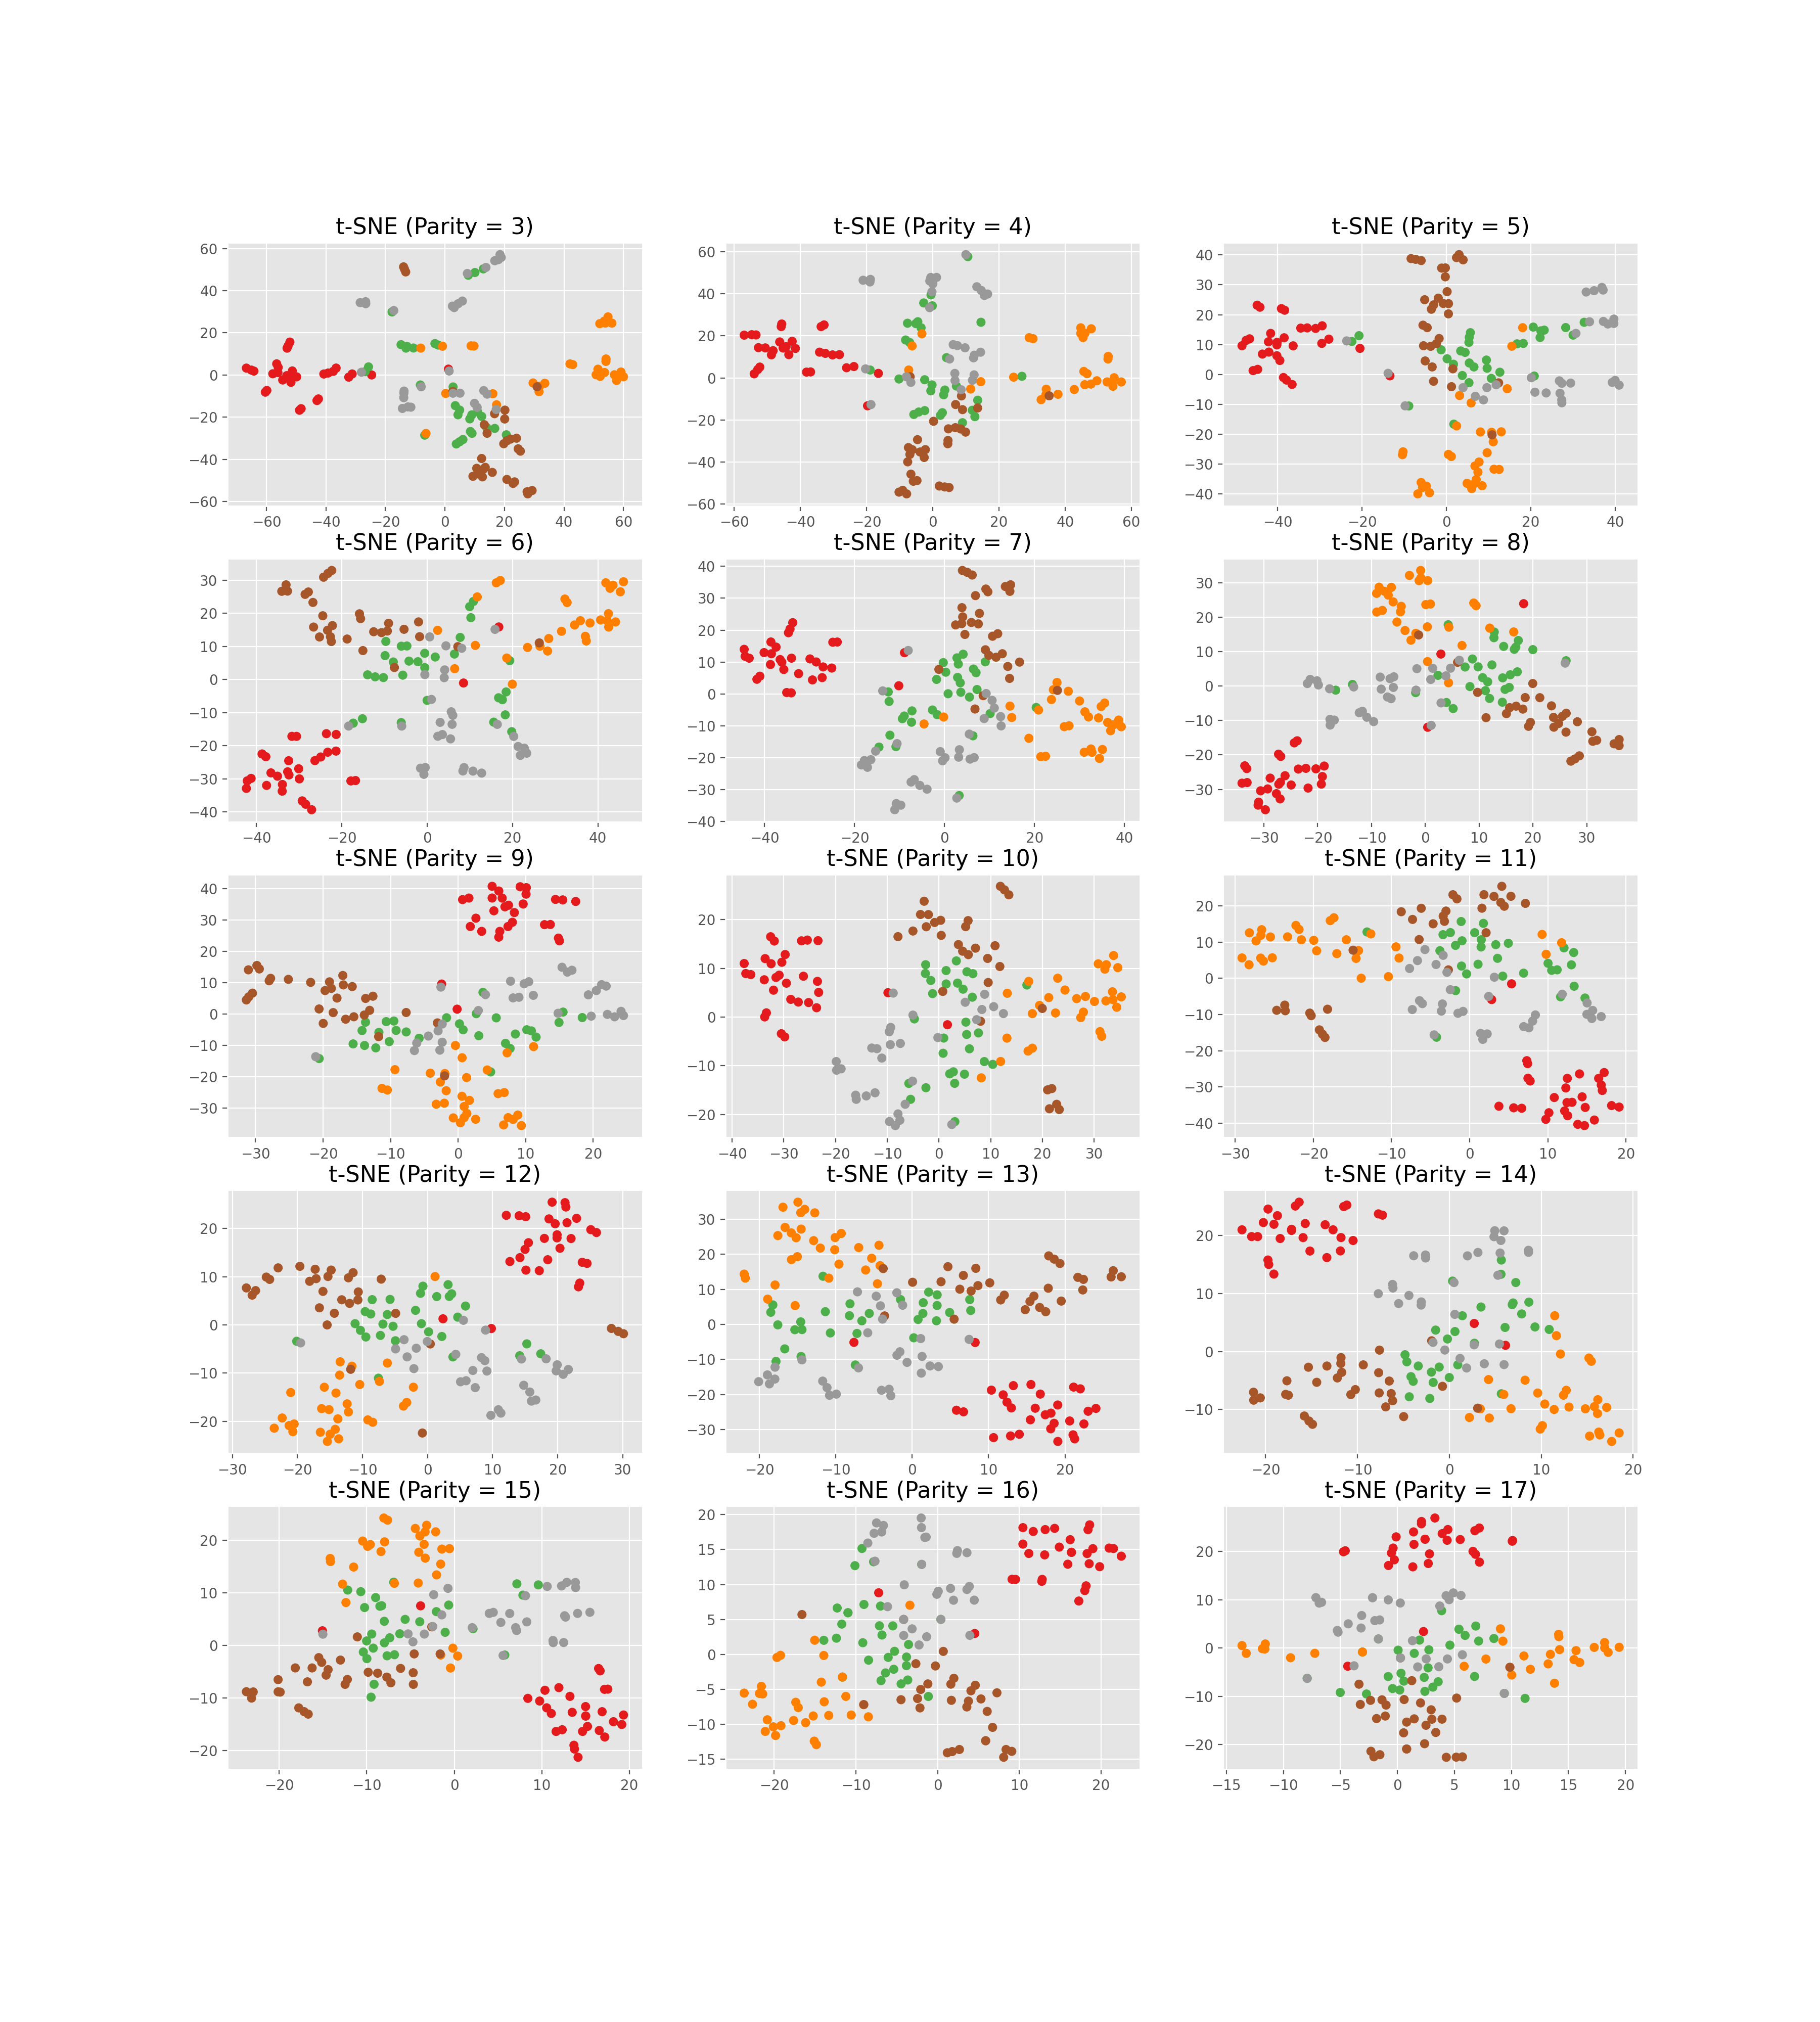
\includegraphics[scale = 0.37]{images/sne_exploration1.png}    
\captionsetup{labelformat=empty}
\vspace{-65pt}
\caption{\scriptsize{Figure 2: t-SNE exploration for perplexity values 3 - 17}}
\end{figure}

\newpage

\begin{figure}[H]
\centering
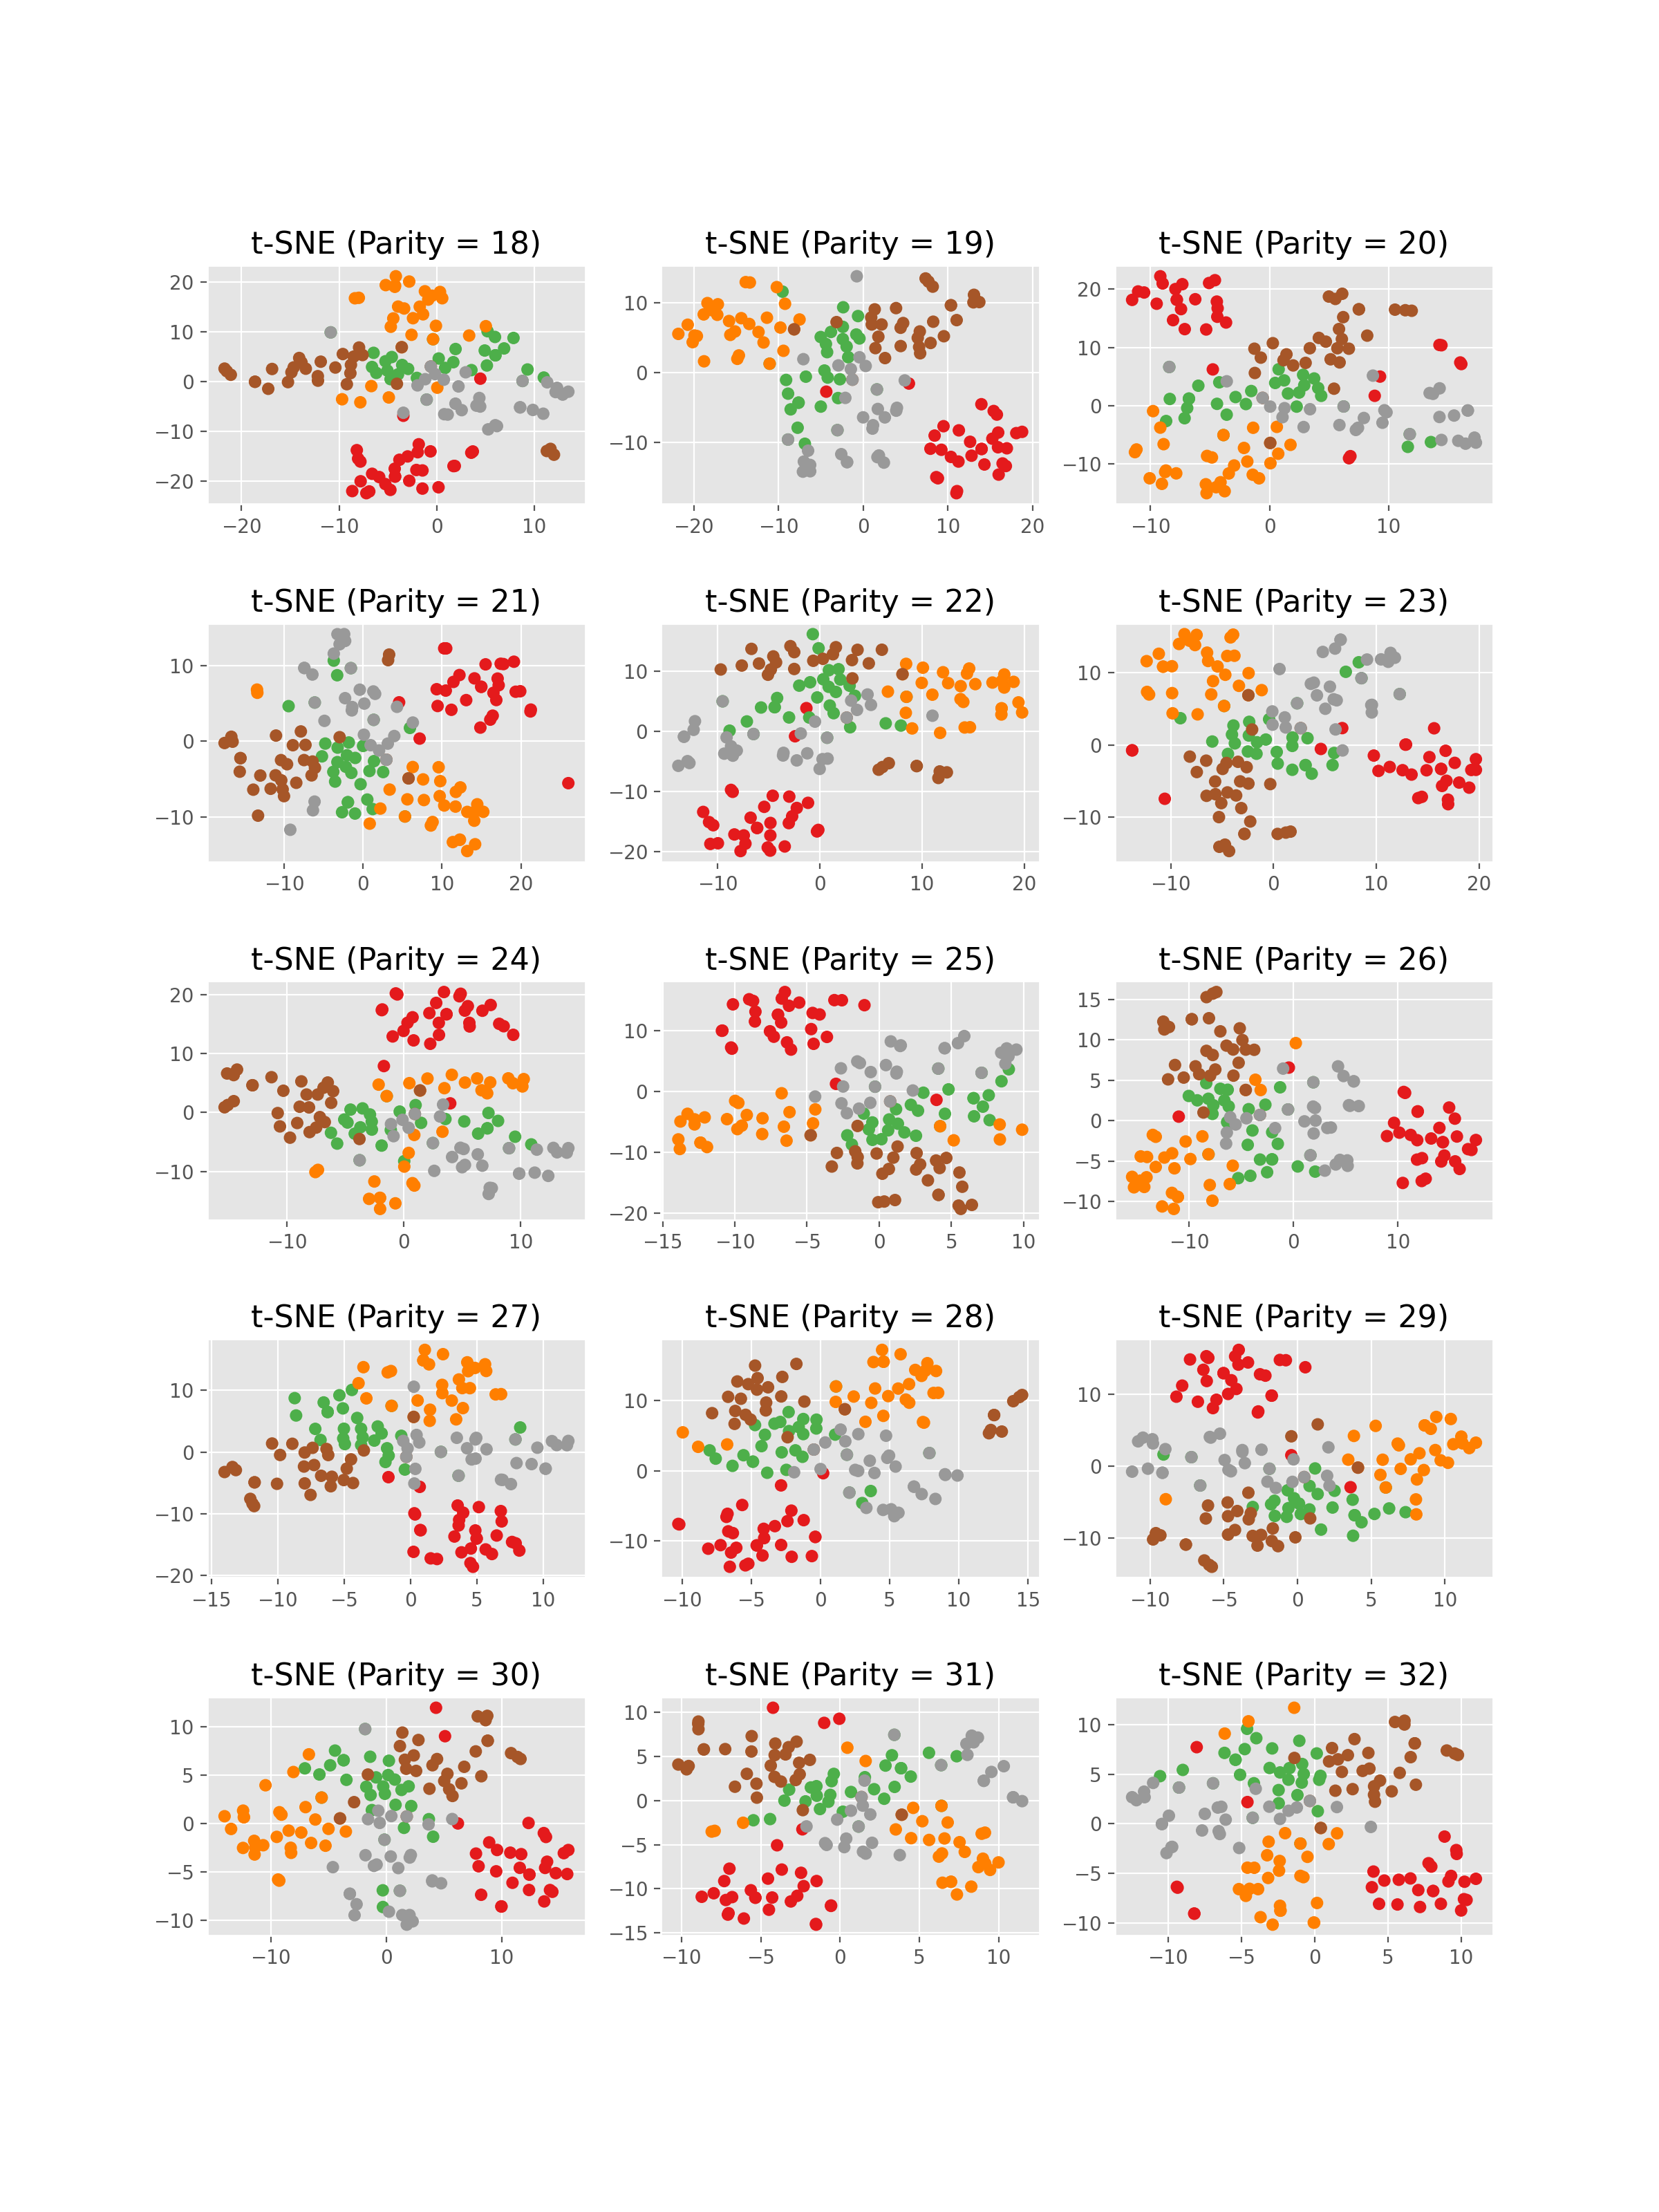
\includegraphics[scale = 0.55]{images/sne_exploration2.png}    
\captionsetup{labelformat=empty}
\vspace{-75pt}
\caption{\scriptsize{Figure 3: t-SNE exploration for perplexity values 18 - 32}}
\end{figure}

\newpage

\begin{figure}[H]
\centering
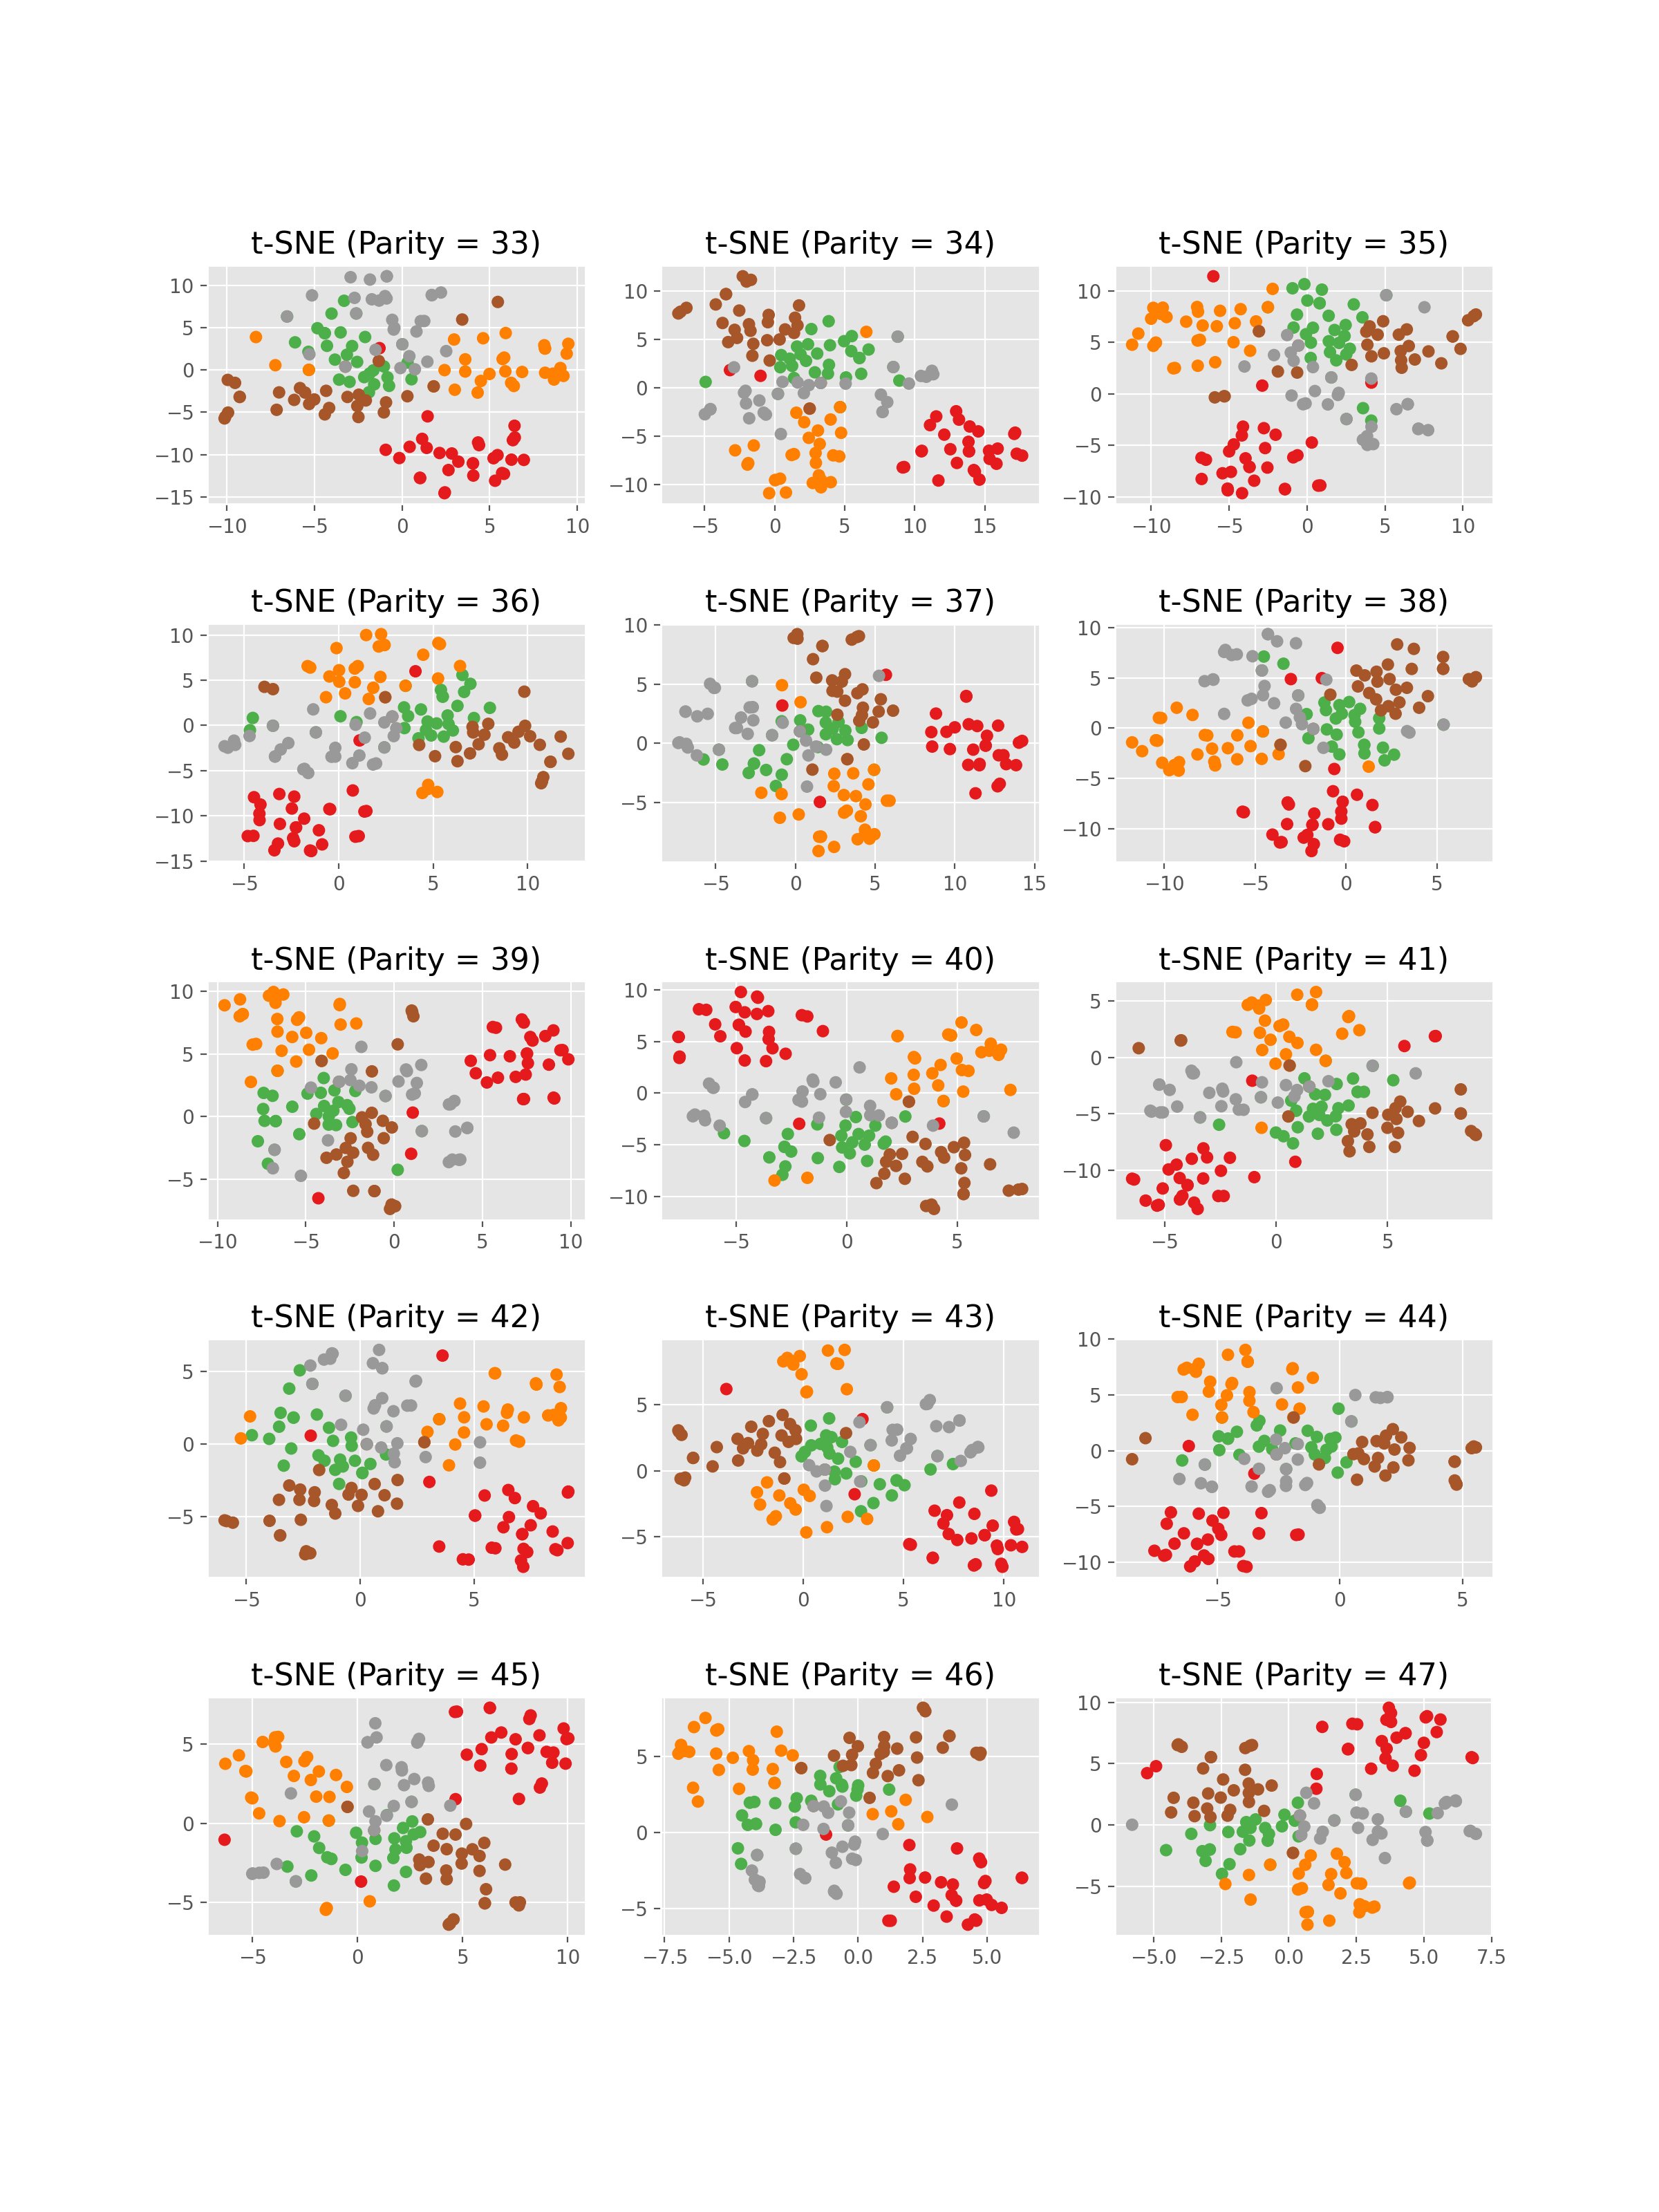
\includegraphics[scale = 0.55]{images/sne_exploration3.png}    
\captionsetup{labelformat=empty}
\vspace{-75pt}
\caption{\scriptsize{Figure 4: t-SNE exploration for perplexity values 33 - 47}}
\end{figure}

\newpage

\begin{figure}[H]
\centering
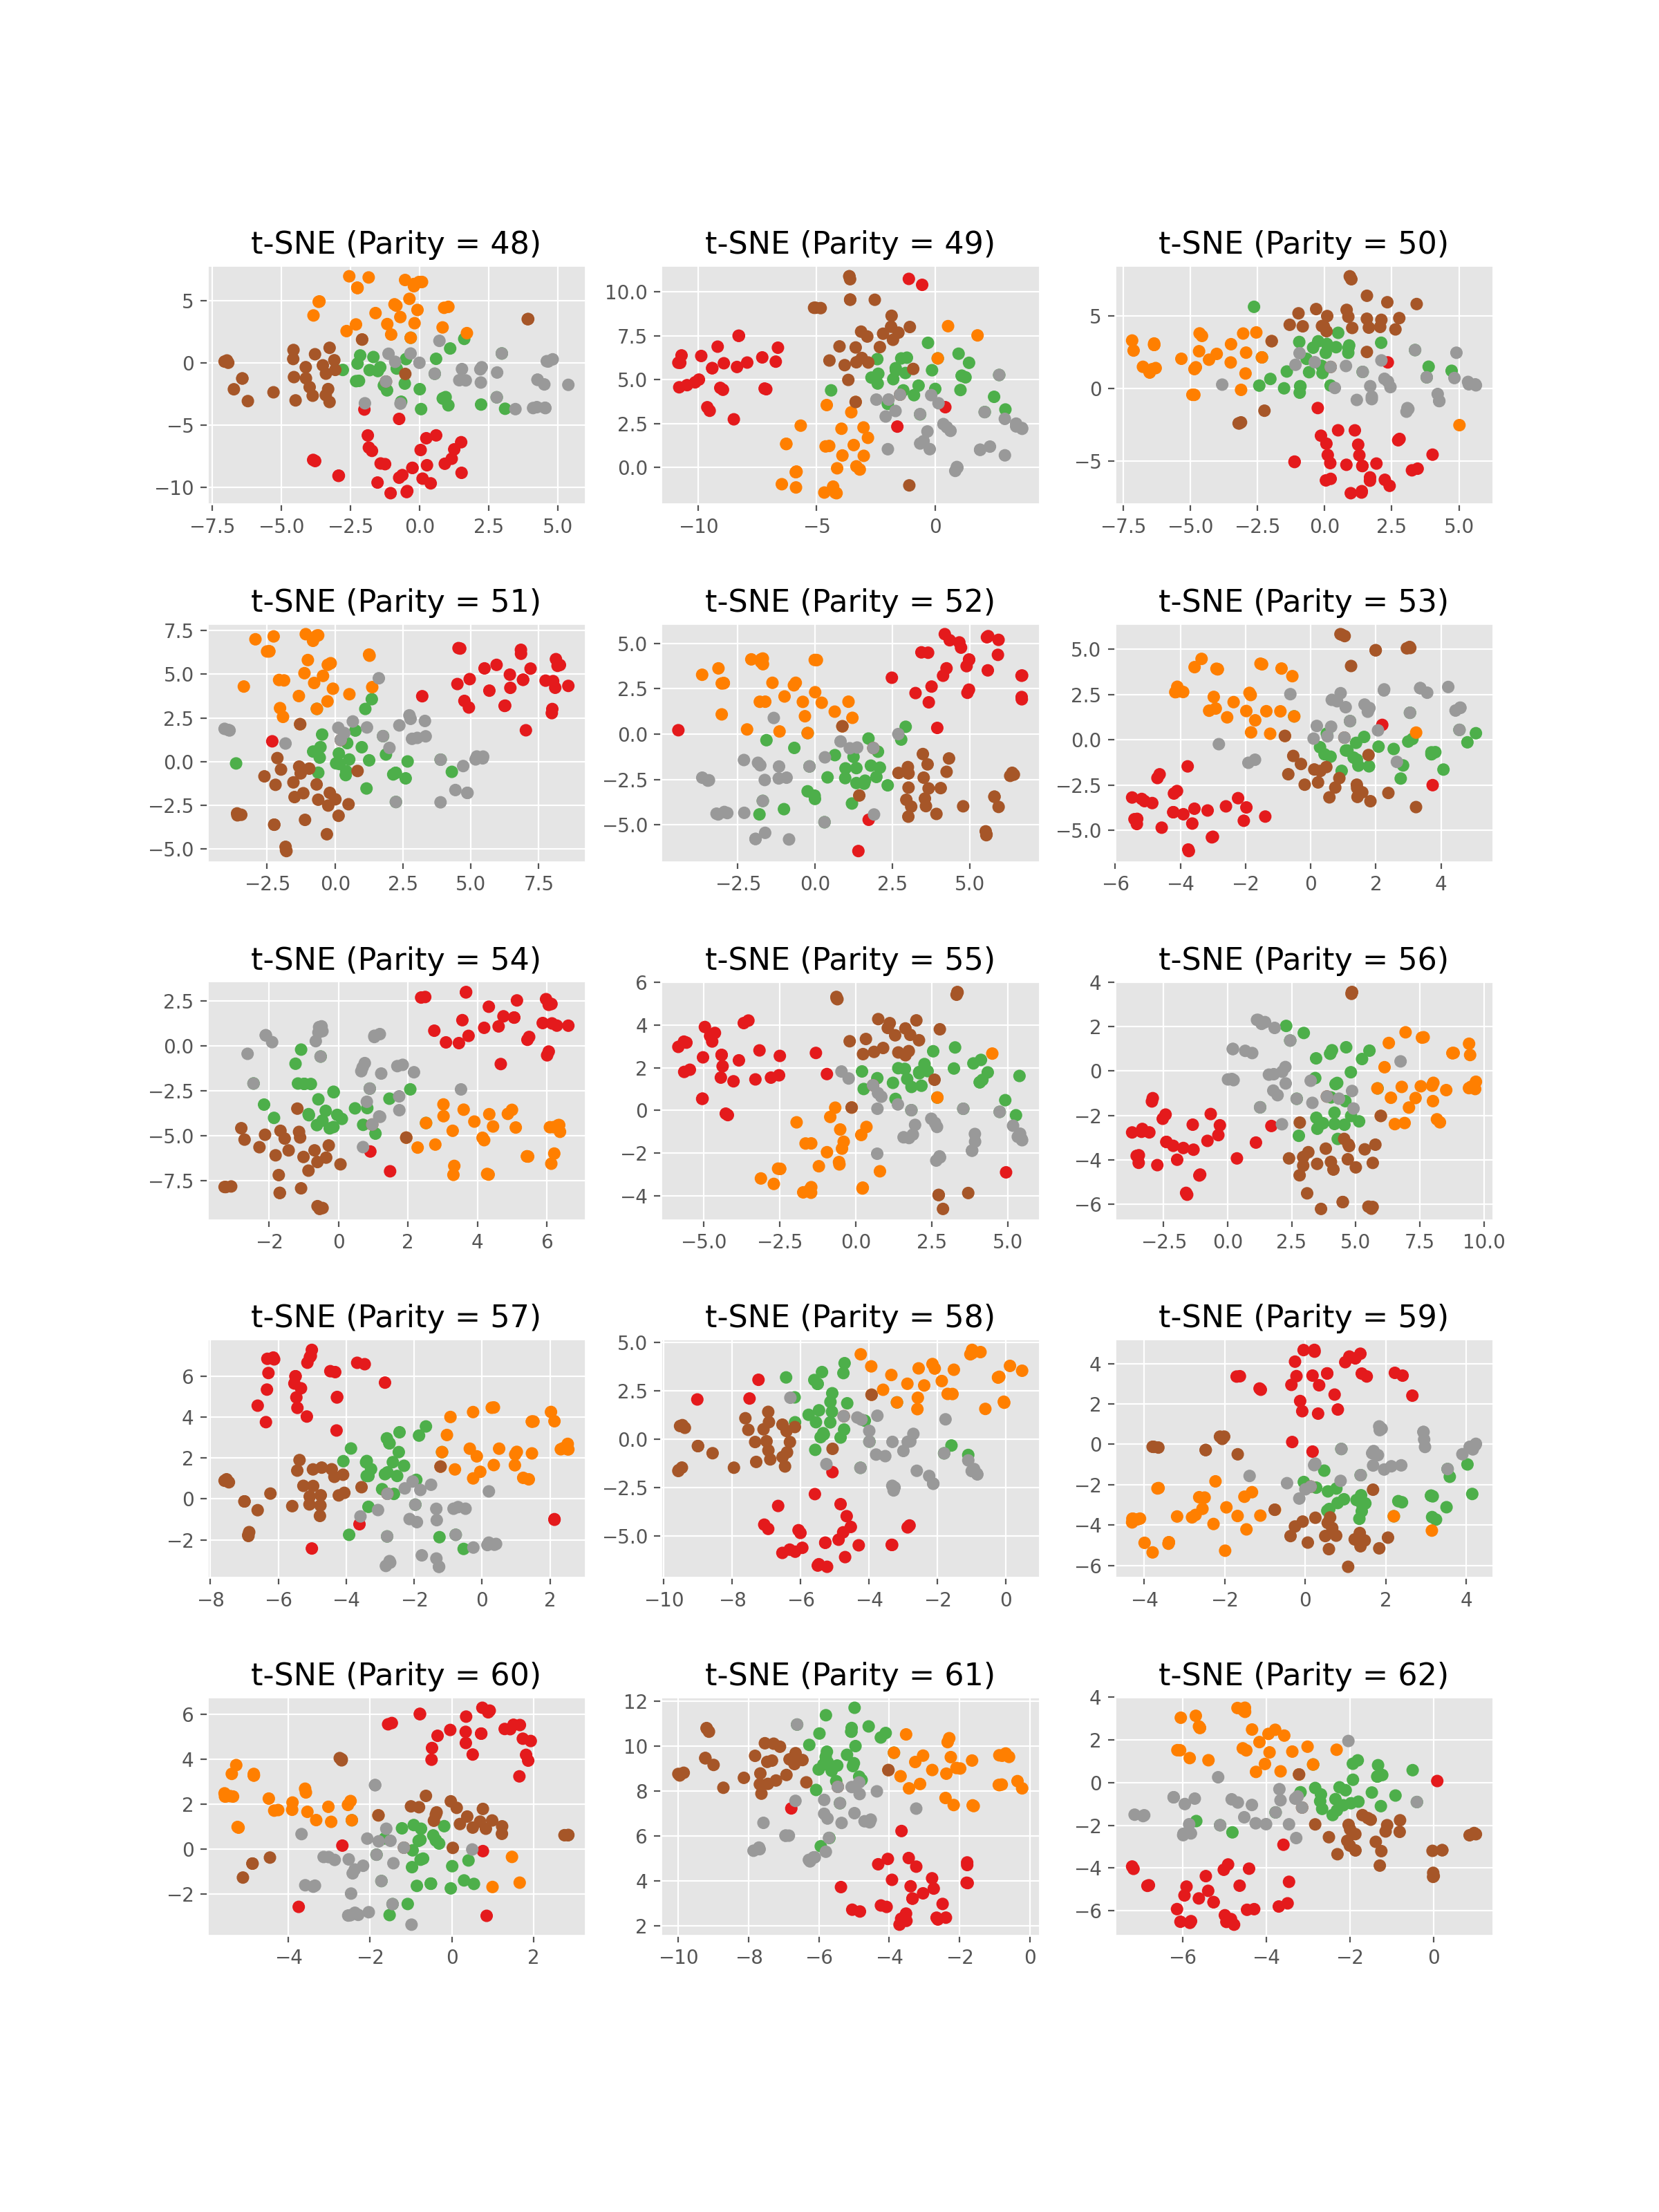
\includegraphics[scale = 0.55]{images/sne_exploration4.png}    
\captionsetup{labelformat=empty}
\vspace{-75pt}
\caption{\scriptsize{Figure 5: t-SNE exploration for perplexity values 48 - 62}}
\end{figure}


\newpage
\textbf{Question 4 (clustering):}\newline
Plot the kmeans objective as a function of k. Do you observe monotonically decreasing objective value as we increase k? Do you see any evidence from this curve that suggests k = 5? Provide an explanation for your results. \newline

\textbf{Response:}\newline
We do observe a monotonically decreasing objective value as we increase k. We would want to look for hitches or elbow points in this graph to use as evidence for optimal k value.  Looking at Figure 6 we see that there are no blatantly standout sharp elbow points -- so we may value multiple elbow points equally with this inspection method. \newline 

Increasing the scale of Figure 6 (Figure 7), we can see there is an elbow point at $k\approx5$. This may provide evidence of to suggest k=5, however like mentioned above it may be hard to pick a "best elbow" point given a lack of clear standout elbow point. Consequentially, we would want to use additional methods to determine if k=5 is a good choice. 
\begin{figure}[H]
\centering
\begin{minipage}{.45\textwidth}
  \centering
  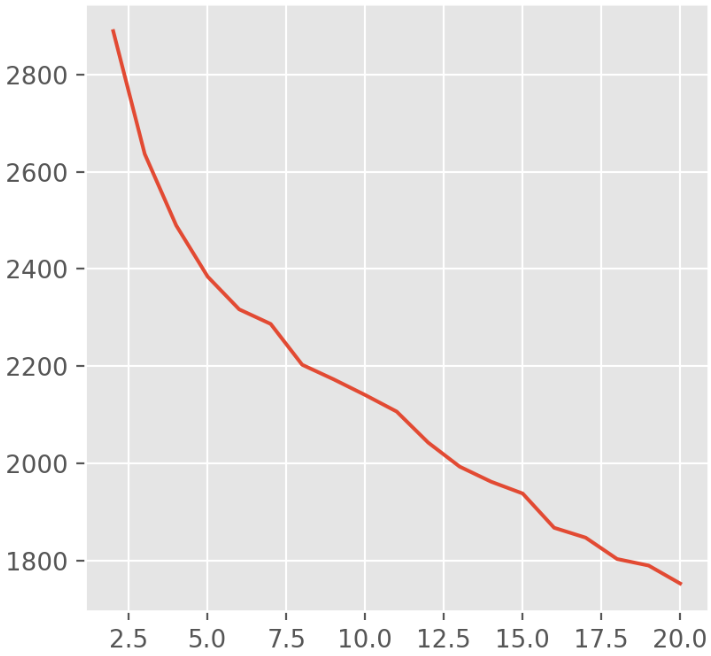
\includegraphics[width=1\linewidth]{images/clustering_inertia_graph.png}
  \captionsetup{labelformat=empty}
  \caption{\scriptsize{Figure 6: kmeans objective as function of k}}
\end{minipage}%%
\hspace{25pt}
\begin{minipage}{.42\textwidth}
  \centering
  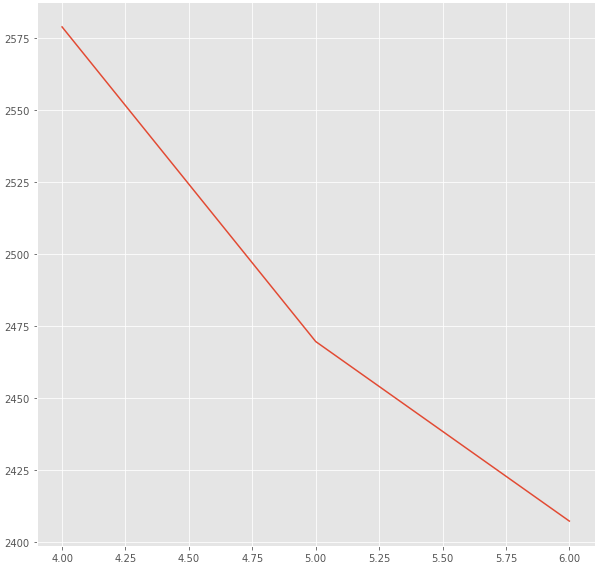
\includegraphics[width=1\linewidth]{images/Zoomed_inertia_graph.png}
  \captionsetup{labelformat=empty}
  \caption{\scriptsize{{Figure 7: Increased scale of Figure 2 around point of interest for visual inspection}}}
\end{minipage}
\end{figure}

\textbf{Question 5 (clustering):} \newline
Plot each metric you get as a function of k. Do you k = 5 gives the best score for different metrics? Provide
an explanation for your observation. Which of these three metrics are appropriate to use if we are evaluating
two different clustering algorithms that automatically search for the number of clusters in the data (that is,
one algorithm might find five clusters in the data while the other might find ten)? \newline
\newpage
\textbf{Response:}\newline

\begin{figure}[H]
\centering
\begin{minipage}{.4\textwidth}
  \centering
  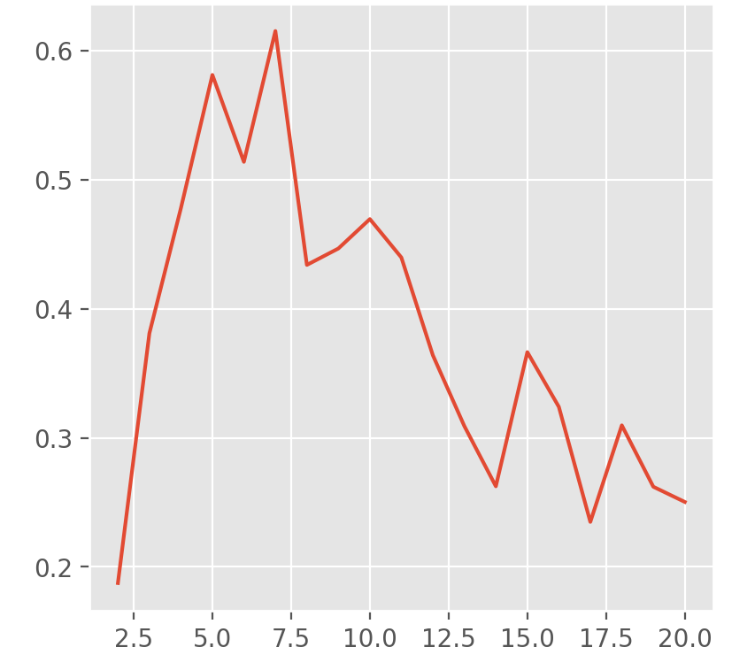
\includegraphics[width=1\linewidth]{images/RAND_graph.png}
  \captionsetup{labelformat=empty}
  \caption{\scriptsize{Figure 8: Adjusted RAND score}}
  \label{fig:test1}
\end{minipage}%%
\vspace{15pt}
\begin{minipage}{.37\textwidth}
  \centering
  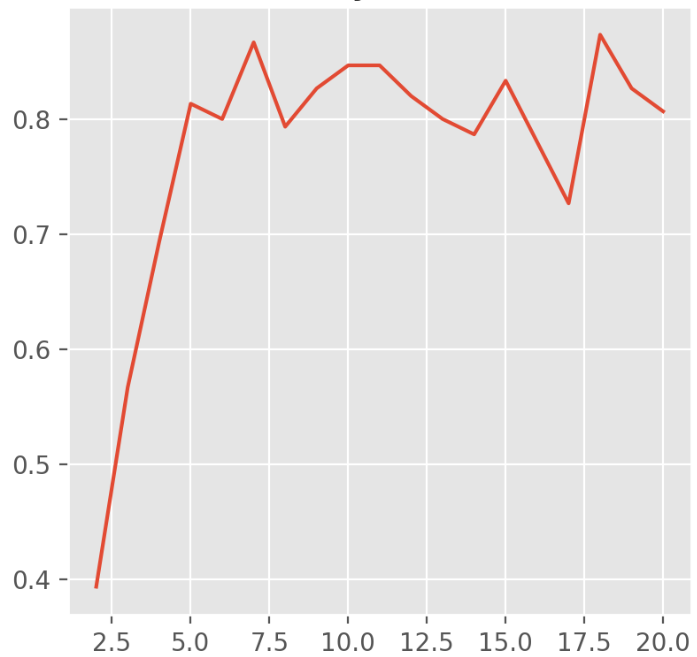
\includegraphics[width=1\linewidth]{images/Purity_graph.png}
  \captionsetup{labelformat=empty}
  \caption{\scriptsize{{Figure 9: Purity score}}}
  \label{fig:test2}
\end{minipage}
\begin{minipage}{.4\textwidth}
  \centering
  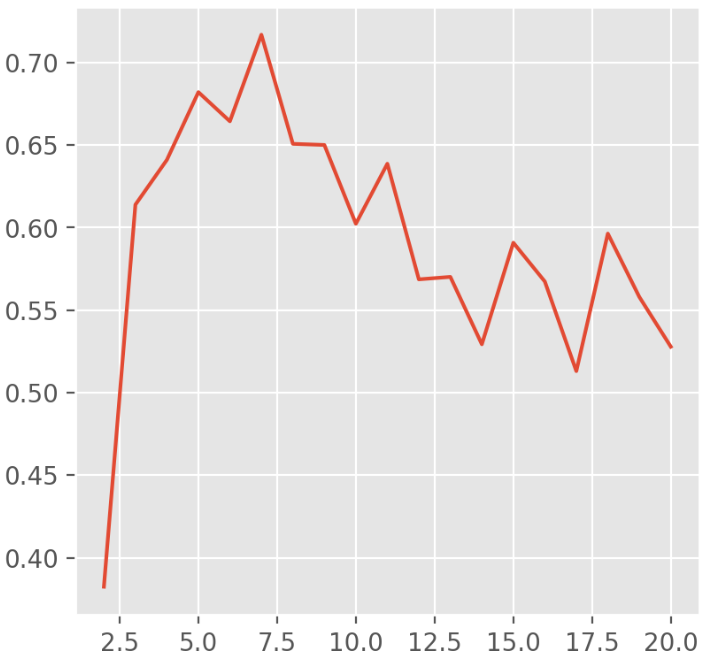
\includegraphics[width=1\linewidth]{images/Mutual_info_graph.png}
  \captionsetup{labelformat=empty}
  \caption{\scriptsize{{Figure 10: Normalized Mutual information score.}}}
  \label{fig:test2}
\end{minipage}
\end{figure}


Figures 8-10 showcases our exploration using RAND, mutual information and purity as functions of k. \newline 

Thinking about purity, we think k=5 gives us fairly good score; however it looks like 7 could potentially be better. We can think of purity s a measure of the extent that a cluster contains a single class.  It is important to note with purity that you can maximize the value by creating the same amount of clusters as there is data. So we must be aware of the amount of data we are evaluating when using this metric.\newline

With the Adjusted RAND we are looking for higher scores. RAND is a metric of similarity, measuring the similarity of two sets of clusters. It determines how similar the elements are. So again K=5 is good but since k=7 is higher, it might be the better choice when viewing this metric. For example 7 clusters may be able to isolate a few more clusters of higher similarity in messy overlap regions.\newline 

Normalized Mutual information is similar to RAND in the sense that it is looking at the the similarity between different cluster sets, it just uses slightly different theory. It the reduction of the entropy class labels. Its essentially telling us how the uncertainty about a given class label may decrease when we know the cluster label. Again a higher mutual information score usually is a indication of better performance, as it correlates to low uncertainty.  So K=7 may be a better choice than k=5 in when using this metric. \newline 

So in general we would probably decide to further explore k=7 since it preforms the best out of those metrics.\newline

We would want to use adjusted RAND and normalized mutual information since those methods are useful for comparing models with different k values, since the metrics do not assume any type of clustering structure. But we do need some understand of ground truth labels, so if we do not have those we would maybe need to use elbow method or some other type of metric like silhouette method \newline
\begin{center} \Large{\textbf{Word Embedding Exploration }} \end{center}

\textbf{Question 1:}\newline
How can you improve the bag-of-words representation for classification using the word embedding?\newline

\textbf{Response:}
For our first exploration we explored using weighted averages. Figure 11 highlights our accuracy for linear SVM using this improvement method. We chose to explore this method because we care about sentences, so it makes sense to add all the embeddings together and then "normalize" it with the average to give us information about the sentence itself. Averaging is important since we want to make sure long sentences are not getting larger weightings just due to length solely. This idea of taking average weights works well for identify similar tweets due to the high dimensionality of the embedding space. A convenient outcome of this high dimensionality is that it is extremely unlikely for two different tweets do have the same average (high dimension nearly always produces orthogonal vectors when randomly chosen), while it is guaranteed two similar tweets will have close average embedding weights. This is the logic behind why average weight is a use full tool\newline


\begin{figure}[H]
\centering
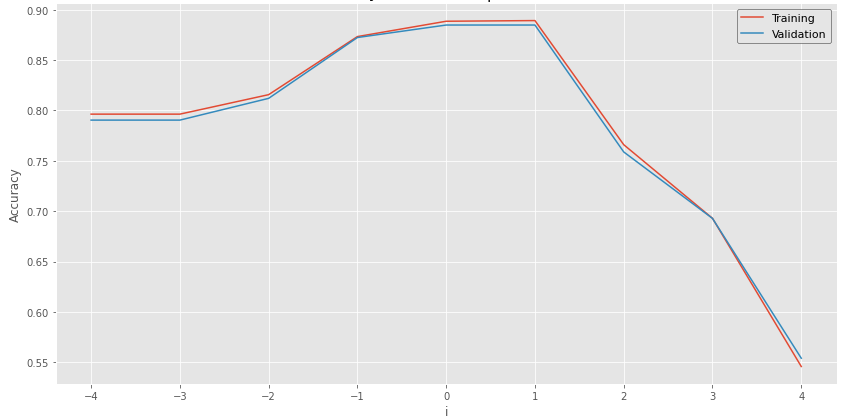
\includegraphics[scale = 0.45]{images/part2_exploration1.png}    
\captionsetup{labelformat=empty}
\vspace{-5pt}
\caption{\scriptsize{\;\;\;\;\;\;\;\;\;\;\;\;\;Figure 11: Linear SVM training and validation accuracy after exploring weighted average word embedding}}
\end{figure}

For our second exploration we tried to reduce the noise of each tweet by removing words in the tweet with "@". Usually they were words like "@UnitedAir" or "@SouthwestAir". We did not see any significant change in our training and validation accuracy.  This told us that these words were not significant sources of noise. \newline


The third approach we took we sort of thought as a "semi-supervised" approach. There are words in our tweets that are not in the vocabulary of the GloVe embedder -- so we may loose valuable information when those words are assigned the 0-embedding. Our idea was to overcome the issue by using another vector representation, which is TFID. We used TFID to vectorize all the words in our tweets and then used kmeans to cluster the them. Afterward, we calculated the GloVe embeddings for these words and computed the weighted average embedding of those clusters using. Note that we left out the words with zero embeddings when calculating the average. Once we determined the weighted average embeddings of the clusters, we then propagated those weighted averages to the words with zero-embeddings in the same clusters. As a result, we might gain some information from words that otherwise would provide zero information. \newline

Unfortunately, we could not get this idea to fully work properly to produce an accuracy graph, but we explored the idea and code thoroughly thinking about this idea and implementation.

\begin{center} \Large{\textbf{General Discussion/Reflection}} \end{center}


This was one of the most applied projects we were tasked with this semester as a team, mostly because it was the most open ended without many "guided" instructions or questions in part 2.  This simulates a real work environment. Our biggest takeaway away -- it is challenging and sometimes frustrating.  We came across various ideas we thought would be great to then realize that they did not improve performance at all. We then had to go back to the drawing board.  It was a good test of our resilience as problems solvers we've been working on this term. \newline

Talking more specifically to the results of this assignment. We found it interesting that removing tweets with "@" did not reduce the noise in our data.  Additionally we were not initially expecting so much variety in our t-SNE perplexity graphs, but then realized how we can arrive at different local minimum.

%

\end{document}